% Generated from reviewed lane; compile via book/textbook.tex.
\clearpage

原书 PDF 页 27；印刷页码 14。

\href{source-images/pdf-027.jpeg}{原页：书页 14／PDF 27}

\section{第 2 章 插值法}\label{ch02a-ux7b2c-2-ux7ae0-ux63d2ux503cux6cd5}

\subsection{2.1 引言}\label{ch02a-ux5f15ux8a00}

许多实际问题都要用函数 \(y=f(x)\) 来表示某种内在规律的数量关系，其中相当一部分函数是通过实验或观测得到的。虽然 \(f(x)\) 在某个区间 \([a,b]\) 上是存在的，有的还是连续的，但却只能给出 \([a,b]\) 上一系列点 \(x_i\) 的函数值 \(y_i=f(x_i)\)（\(i=0,1,\cdots,n\)），这只是一张函数表。有的函数虽有解析表达式，但由于计算复杂，使用不方便，通常也造一个函数表，如大家熟悉的三角函数表、对数表、平方根和立方根表等。为了研究函数的变化规律，往往需要求出不在表上的函数值。因此，我们希望根据给定的函数表构造一个既能反映函数 \(f(x)\) 的特性、又便于计算的简单函数 \(P(x)\)，用 \(P(x)\) 近似 \(f(x)\)。通常选一类较简单的函数如代数多项式或分段代数多项式作为 \(P(x)\)，并使 \(P(x_i)=f(x_i)\) 对于 \(i=0,1,\cdots,n\) 成立，这样确定的 \(P(x)\) 就是我们希望得到的插值函数。例如，在现代机械工业中用计算机程序控制加工机械零件，根据设计可给出零件外形曲线的某些型值点 \((x_i,y_i)\)（\(i=0,1,\cdots,n\)），加工时为控制每步走刀方向及步数，就要算出零件外形曲线其他点的函数值，才能加工出外表光滑的零件，这就是求插值函数的问题。下面给出有关插值法的定义。

\textbf{定义 2.1} 设函数 \(y=f(x)\) 在区间 \([a,b]\) 上有定义，且已知在点 \(a\le x_0\le x_1<\cdots<x_n\le b\) 上的值 \(y_0,y_1,\cdots,y_n\)，若存在一简单函数 \(P(x)\)，使

\[
P(x_i)=y_i\qquad (i=0,1,\cdots,n)
\tag{2.1.1}
\]

成立，就称 \(P(x)\) 为 \(f(x)\) 的\textbf{插值函数}。点 \(x_0,x_1,\cdots,x_n\) 称为\textbf{插值节点}，包含插值节点的区间 \([a,b]\) 称为\textbf{插值区间}，求插值函数 \(P(x)\) 的方法称为\textbf{插值法}。若 \(P(x)\) 是次数不超过 \(n\) 的代数多项式，即

\[
P(x)=a_0+a_1x+\cdots+a_nx^n,
\tag{2.1.2}
\]

其中 \(a_i\) 为实数，就称 \(P(x)\) 为\textbf{插值多项式}，相应的插值法称为\textbf{多项式插值}；若 \(P(x)\) 为分段的多项式，就称之为\textbf{分段插值}；若 \(P(x)\) 为三角多项式，就称之为\textbf{三角插值}。本章只讨论多项式插值与分段插值。

从几何图形上看，插值法就是求曲线 \(y=P(x)\)，使其通过给定的 \(n+1\) 个点 \((x_i,y_i)\)，\(i=0,1,\cdots,n\)，并用它近似已知曲线 \(y=f(x)\)，如图 2.1 所示。

插值法是一种古老的数学方法，它来自生产实践。早在一千多年前，我国科学家在研究历法中就应用了线性插值与二次插值，但它的基本理论和结果却是在微积分

\begin{quote}
本页末句续 PDF 28。
\end{quote}

\subsubsection{校注（agent 补充）：NA5E-E001}\label{ch02a-ux6821ux6ce8agent-ux8865ux5145na5e-e001}

扫描原页中，定义 2.1 的前两个节点确实印为 \(x_0\le x_1\)；这里忠实保留。它与 2.2.1 证明中``\(i\ne j\) 时 \(x_i\ne x_j\)''的前提不一致。普通 Lagrange 插值存在唯一性要求节点互异，使用时应采用

\[
a\le x_0<x_1<\cdots<x_n\le b.
\]

核验反例：当 \(n=1\)、\(x_0=x_1=0\)、\(y_0=y_1=c\) 时，所有 \(P(x)=c+tx\)（任意实数 \(t\)）都满足节点条件，故不唯一。这里的严格不等号是有明确依据的校注，不能把它当作原书实际印字。

\clearpage

原书 PDF 页 28；印刷页码 15。

\href{source-images/pdf-028.jpeg}{原页：书页 15／PDF 28}

\begin{quote}
页首接 PDF 27 的``微积分''。
\end{quote}

产生以后才逐步完善的，其应用也日益增多。特别是在电子计算机广泛使用以后，由于航空、造船、精密机械加工等实际问题的需要，插值法在实践上和理论上显得更为重要，由此得到进一步发展，尤其是近几十年发展起来的样条（spline）插值，获得了更为广泛的应用。

本章主要研究如何求出插值函数（包括分段插值函数及样条插值函数），并讨论插值函数 \(P(x)\) 的存在唯一性、收敛性及误差估计等。


\includegraphics[width=0.85\linewidth,height=\textheight,keepaspectratio,alt={图 2.1（原图裁切）}]{verified/assets/ch02a/figure-2.1.png}

图 2.1（原图）：曲线 \(y=P(x)\) 与 \(y=f(x)\) 通过共同的插值节点。全部文字标签：\(y\)、\(x\)、\(O\)、\(x_1\)、\(x_n\)、\(y_1\)、\(y_n\)、\(y=f(x)\)、\(y=P(x)\)。

\subsection{2.2 Lagrange 插值}\label{ch02a-lagrange-ux63d2ux503c}

\subsubsection{2.2.1 插值多项式的存在唯一性}\label{ch02a-ux63d2ux503cux591aux9879ux5f0fux7684ux5b58ux5728ux552fux4e00ux6027}

设 \(P(x)\) 是形如式（2.1.2）的插值多项式，用 \(H_n\) 代表所有次数不超过 \(n\) 的多项式集合，于是 \(P(x)\in H_n\)（符号 \(\in\) 表示属于）。所谓插值多项式 \(P(x)\) 存在唯一，就是指在集合 \(H_n\) 中有且只有一个 \(P(x)\) 满足式（2.1.1）。由式（2.1.1）可得

\[
\begin{cases}
a_0+a_1x_0+\cdots+a_nx_0^n=y_0,\\
a_0+a_1x_1+\cdots+a_nx_1^n=y_1,\\
\qquad\qquad\vdots\\
a_0+a_1x_n+\cdots+a_nx_n^n=y_n.
\end{cases}
\tag{2.2.1}
\]

这是一个关于 \(a_0,a_1,\cdots,a_n\) 的 \(n+1\) 元线性方程组。要证明插值多项式的存在唯一，只要证明方程组（2.2.1）的解存在唯一，也就是证明方程组（2.2.1）的系数行列式

\[
V_n(x_0,x_1,\cdots,x_n)=
\begin{vmatrix}
1 & x_0 & x_0^2 & \cdots & x_0^n\\
1 & x_1 & x_1^2 & \cdots & x_1^n\\
\vdots & \vdots & \vdots & & \vdots\\
1 & x_n & x_n^2 & \cdots & x_n^n
\end{vmatrix}
\tag{2.2.2}
\]

不为零，其中 \(V_n(x_0,x_1,\cdots,x_n)\) 称为 Vandermonde 行列式。利用行列式性质可得

\[
V_n(x_0,x_1,\cdots,x_n)
=\prod_{i=1}^{n}\prod_{j=0}^{i-1}(x_i-x_j),
\]

由于 \(i\ne j\) 时 \(x_i\ne x_j\)，上式所有因子 \(x_i-x_j\ne0\)，于是 \(V_n(x_0,x_1,\cdots,x_n)\ne0\)，故方程组（2.2.1）存在唯一的一组解 \(a_0,a_1,\cdots,a_n\)。以上论述可写成如下定理。

\textbf{定理 2.1} 满足条件式（2.1.1）的插值多项式（2.1.2）存在唯一。

\clearpage

原书 PDF 页 29；印刷页码 16。

\href{source-images/pdf-029.jpeg}{原页：书页 16／PDF 29}

\subsubsection{2.2.2 线性插值与抛物插值}\label{ch02a-ux7ebfux6027ux63d2ux503cux4e0eux629bux7269ux63d2ux503c}

从定理 2.1 的证明可看到，要求插值多项式 \(P(x)\)，可以通过求方程组（2.2.1）的解 \(a_0,a_1,\cdots,a_n\) 得到。但这样做不但计算复杂，且难以得到 \(P(x)\) 的简单表达式。为了求得便于使用的简单的插值多项式 \(P(x)\)，先讨论 \(n=1\) 的情形。

假定已知区间 \([x_k,x_{k+1}]\) 的端点处的函数值 \(y_k=f(x_k)\)，\(y_{k+1}=f(x_{k+1})\)，要求线性插值多项式 \(L_1(x)\)，使它满足

\[
L_1(x_k)=y_k,\qquad L_1(x_{k+1})=y_{k+1}.
\]

\(y=L_1(x)\) 的几何意义就是通过两点 \((x_k,y_k)\) 和 \((x_{k+1},y_{k+1})\) 的直线，如图 2.2 所示。\(L_1(x)\) 的表达式可由几何意义直接给出，即

\[
L_1(x)=y_k+\frac{y_{k+1}-y_k}{x_{k+1}-x_k}(x-x_k)
\quad\text{（点斜式）},
\tag{2.2.3}
\]

\[
L_1(x)=\frac{x_{k+1}-x}{x_{k+1}-x_k}y_k
+\frac{x-x_k}{x_{k+1}-x_k}y_{k+1}
\quad\text{（两点式）}.
\tag{2.2.4}
\]


\includegraphics[width=0.85\linewidth,height=\textheight,keepaspectratio,alt={图 2.2（原图裁切）}]{verified/assets/ch02a/figure-2.2.png}

图 2.2（原图）：直线 \(y=L_1(x)\) 与曲线 \(y=f(x)\) 在两节点相交。全部文字标签：\(y\)、\(x\)、\(O\)、\(x_k\)、\(x_{k+1}\)、\(y_k\)、\(y_{k+1}\)、\(y=L_1(x)\)、\(y=f(x)\)。

由两点式方程看出，\(L_1(x)\) 是由两个线性函数

\[
l_k(x)=\frac{x-x_{k+1}}{x_k-x_{k+1}},
\qquad
l_{k+1}(x)=\frac{x-x_k}{x_{k+1}-x_k}
\]

的线性组合得到的，其系数分别为 \(y_k\) 及 \(y_{k+1}\)，即

\[
L_1(x)=y_kl_k(x)+y_{k+1}l_{k+1}(x).
\tag{2.2.5}
\]

显然，\(l_k(x)\) 及 \(l_{k+1}(x)\) 也是线性插值多项式，在节点 \(x_k\) 及 \(x_{k+1}\) 上满足条件

\[
l_k(x_k)=1,\quad l_k(x_{k+1})=0,\quad
l_{k+1}(x_k)=0,\quad l_{k+1}(x_{k+1})=1.
\]

称函数 \(l_k(x)\) 及 \(l_{k+1}(x)\) 为\textbf{一次插值基函数}或\textbf{线性插值基函数}，它们的图形分别如图 2.3(a)、(b) 所示。


\includegraphics[width=0.85\linewidth,height=\textheight,keepaspectratio,alt={图 2.3（原图裁切）}]{verified/assets/ch02a/figure-2.3.png}

图 2.3（原图）：(a) \(l_k(x)\) 在 \(x_k\) 处为 \(1\)，在 \(x_{k+1}\) 处为 \(0\)；(b) \(l_{k+1}(x)\) 在 \(x_k\) 处为 \(0\)，在 \(x_{k+1}\) 处为 \(1\)。两图全部文字标签：\(y\)、\(x\)、\(O\)、\(1\)、\(x_k\)、\(x_{k+1}\)、\(l_k(x)\)、\(l_{k+1}(x)\)、(a)、(b)。

下面讨论 \(n=2\) 的情况。假定插值节点为 \(x_{k-1},x_k,x_{k+1}\)，要求二次插值多项式 \(L_2(x)\)，使它满足

\begin{quote}
页末插值条件续 PDF 30。
\end{quote}

\clearpage

原书 PDF 页 30；印刷页码 17。

\href{source-images/pdf-030.jpeg}{原页：书页 17／PDF 30}

\begin{quote}
页首承接 PDF 29 的二次插值条件；末式展开续 PDF 31。
\end{quote}

\[
L_2(x_j)=y_j\qquad(j=k-1,k,k+1).
\]

我们知道，\(y=L_2(x)\) 在几何上就是通过三点 \((x_{k-1},y_{k-1})\)、\((x_k,y_k)\)、\((x_{k+1},y_{k+1})\) 的抛物线。为了求出 \(L_2(x)\) 的表达式，可采用基函数方法，此时基函数 \(l_{k-1}(x),l_k(x)\) 及 \(l_{k+1}(x)\) 是二次函数，且在节点上满足条件

\[
\begin{cases}
l_{k-1}(x_{k-1})=1,\quad l_{k-1}(x_j)=0\quad(j=k,k+1),\\
l_k(x_k)=1,\quad l_k(x_j)=0\quad(j=k-1,k+1),\\
l_{k+1}(x_{k+1})=1,\quad l_{k+1}(x_j)=0\quad(j=k-1,k).
\end{cases}
\tag{2.2.6}
\]

满足条件式（2.2.6）的插值基函数是很容易求出的，例如求 \(l_{k-1}(x)\)，因它有两个零点 \(x_k\) 及 \(x_{k+1}\)，故可表示为

\[
l_{k-1}(x)=A(x-x_k)(x-x_{k+1}),
\]

其中 \(A\) 为待定系数，可由条件 \(l_{k-1}(x_{k-1})=1\) 定出，即

\[
A=\frac{1}{(x_{k-1}-x_k)(x_{k-1}-x_{k+1})},
\]

故

\[
l_{k-1}(x)=
\frac{(x-x_k)(x-x_{k+1})}
{(x_{k-1}-x_k)(x_{k-1}-x_{k+1})}.
\]

同理，

\[
l_k(x)=
\frac{(x-x_{k-1})(x-x_{k+1})}
{(x_k-x_{k-1})(x_k-x_{k+1})},
\qquad
l_{k+1}(x)=
\frac{(x-x_{k-1})(x-x_k)}
{(x_{k+1}-x_{k-1})(x_{k+1}-x_k)}.
\]

函数 \(l_{k-1}(x),l_k(x),l_{k+1}(x)\) 称为\textbf{二次插值基函数}或\textbf{抛物插值基函数}，它们在区间 \([x_{k-1},x_{k+1}]\) 上的图形分别如图 2.4(a)、(b)、(c) 所示。


\includegraphics[width=0.85\linewidth,height=\textheight,keepaspectratio,alt={图 2.4（原图裁切）}]{verified/assets/ch02a/figure-2.4.png}

图 2.4（原图）：(a) \(l_{k-1}(x)\)，(b) \(l_k(x)\)，(c) \(l_{k+1}(x)\)，分别在对应节点取 \(1\)、其他两个节点取 \(0\)；左右基函数在部分区间为负。三图全部文字标签：\(y\)、\(x\)、\(O\)、\(1\)、\(x_{k-1}\)、\(x_k\)、\(x_{k+1}\)、\(l_{k-1}(x)\)、\(l_k(x)\)、\(l_{k+1}(x)\)、(a)、(b)、(c)。

利用二次插值基函数 \(l_{k-1}(x),l_k(x),l_{k+1}(x)\)，立即可得到二次插值多项式

\[
L_2(x)=y_{k-1}l_{k-1}(x)+y_kl_k(x)+y_{k+1}l_{k+1}(x),
\tag{2.2.7}
\]

显然，它满足条件

\[
L_2(x_j)=y_j\qquad(j=k-1,k,k+1).
\]

将上面求得的 \(l_{k-1}(x),l_k(x),l_{k+1}(x)\) 代入式（2.2.7），得

\clearpage

原书 PDF 页 31；印刷页码 18。

\href{source-images/pdf-031.jpeg}{原页：书页 18／PDF 31}

\begin{quote}
页首续 PDF 30 的式（2.2.7）展开；页末公式续 PDF 32。
\end{quote}

\[
\begin{aligned}
L_2(x)={}&y_{k-1}
\frac{(x-x_k)(x-x_{k+1})}
{(x_{k-1}-x_k)(x_{k-1}-x_{k+1})}\\
&+y_k
\frac{(x-x_{k-1})(x-x_{k+1})}
{(x_k-x_{k-1})(x_k-x_{k+1})}\\
&+y_{k+1}
\frac{(x-x_{k-1})(x-x_k)}
{(x_{k+1}-x_{k-1})(x_{k+1}-x_k)}.
\end{aligned}
\]

\subsubsection{2.2.3 Lagrange 插值多项式}\label{ch02a-lagrange-ux63d2ux503cux591aux9879ux5f0f}

上面对 \(n=1\) 及 \(n=2\) 的情况，得到了一次与二次插值多项式 \(L_1(x)\) 及 \(L_2(x)\)，它们分别由式（2.2.5）和式（2.2.7）表示。这种用插值基函数表示的方法容易推广到一般情形。下面讨论通过 \(n+1\) 个节点 \(x_0<x_1<\cdots<x_n\) 的 \(n\) 次插值多项式 \(L_n(x)\)，假定它满足条件

\[
L_n(x_j)=y_j\qquad(j=0,1,\cdots,n).
\tag{2.2.8}
\]

为了构造 \(L_n(x)\)，先定义 \(n\) 次插值基函数。

\textbf{定义 2.2} 若 \(n\) 次多项式 \(l_j(x)\)（\(j=0,1,\cdots,n\)）在 \(n+1\) 个节点 \(x_0<x_1<\cdots<x_n\) 上满足条件

\[
l_j(x_k)=
\begin{cases}
1,&k=j,\\
0,&k\ne j
\end{cases}
\qquad(j,k=0,1,\cdots,n),
\tag{2.2.9}
\]

就称这 \(n+1\) 个 \(n\) 次多项式 \(l_0(x),l_1(x),\cdots,l_n(x)\) 为节点 \(x_0,x_1,\cdots,x_n\) 上的 \textbf{\(n\) 次插值基函数}。

\(n=1\) 及 \(n=2\) 时的情况前面已经讨论。用类似的推导方法，可得到 \(n\) 次插值基函数为

\[
l_k(x)=
\frac{(x-x_0)\cdots(x-x_{k-1})(x-x_{k+1})\cdots(x-x_n)}
{(x_k-x_0)\cdots(x_k-x_{k-1})(x_k-x_{k+1})\cdots(x_k-x_n)}
\quad(k=0,1,\cdots,n).
\tag{2.2.10}
\]

显然它满足条件（2.2.9）。于是，满足条件（2.2.8）的插值多项式 \(L_n(x)\) 可表示为

\[
L_n(x)=\sum_{k=0}^{n}y_kl_k(x).
\tag{2.2.11}
\]

由 \(l_k(x)\) 的定义知

\[
L_n(x_j)=\sum_{k=0}^{n}y_kl_k(x_j)=y_j
\qquad(j=0,1,\cdots,n).
\]

形如式（2.2.11）的插值多项式 \(L_n(x)\) 称为 \textbf{Lagrange 插值多项式}，而式（2.2.5）和式（2.2.7）是其 \(n=1\) 和 \(n=2\) 的特殊情形。若引入记号

\[
\omega_{n+1}(x)=(x-x_0)(x-x_1)\cdots(x-x_n),
\tag{2.2.12}
\]

容易求得

\[
\omega'_{n+1}(x_k)
=(x_k-x_0)\cdots(x_k-x_{k-1})(x_k-x_{k+1})\cdots(x_k-x_n),
\]

于是式（2.2.11）可改写成

\clearpage

原书 PDF 页 32；印刷页码 19。

\href{source-images/pdf-032.jpeg}{原页：书页 19／PDF 32}

\begin{quote}
页首接 PDF 31；页末线性插值余项续 PDF 33。
\end{quote}

\[
L_n(x)=\sum_{k=0}^{n}y_k
\frac{\omega_{n+1}(x)}
{(x-x_k)\omega'_{n+1}(x_k)}.
\tag{2.2.13}
\]

注意，\(n\) 次插值多项式 \(L_n(x)\) 通常是次数为 \(n\) 的多项式，特殊情况次数可能小于 \(n\)。例如，通过三点 \((x_0,y_0),(x_1,y_1),(x_2,y_2)\) 的二次插值多项式 \(L_2(x)\)，如果三点共线，则 \(y=L_2(x)\) 就是一直线，而不是抛物线，这时 \(L_2(x)\) 是一次式。

\subsubsection{2.2.4 插值余项}\label{ch02a-ux63d2ux503cux4f59ux9879}

若在 \([a,b]\) 上用 \(L_n(x)\) 近似 \(f(x)\)，则其截断误差为 \(R_n(x)=f(x)-L_n(x)\)，\(R_n(x)\) 也称为插值多项式的余项或插值余项。关于插值余项估计有以下定理。

\textbf{定理 2.2} 设 \(f^{(n)}(x)\) 在 \([a,b]\) 上连续，\(f^{(n+1)}(x)\) 在 \((a,b)\) 内存在，节点 \(a\le x_0<x_1<\cdots<x_n\le b\)，\(L_n(x)\) 是满足条件式（2.2.8）的插值多项式，则对于任何 \(x\in[a,b]\)，插值余项

\[
R_n(x)=f(x)-L_n(x)=\frac{f^{(n+1)}(\xi)}{(n+1)!}\omega_{n+1}(x).
\tag{2.2.14}
\]

这里，\(\xi\in(a,b)\) 且依赖于 \(x\)，\(\omega_{n+1}(x)\) 是式（2.2.12）所定义的。

\textbf{证明} 由给定条件知，\(R_n(x)\) 在节点 \(x_k\)（\(k=0,1,\cdots,n\)）上为零，即

\[
R_n(x_k)=0\qquad(k=0,1,\cdots,n),
\]

于是

\[
R_n(x)=K(x)(x-x_0)(x-x_1)\cdots(x-x_n)=K(x)\omega_{n+1}(x),
\tag{2.2.15}
\]

其中 \(K(x)\) 是与 \(x\) 有关的待定函数。

现把 \(x\) 看成 \([a,b]\) 上一个固定点，作函数

\[
\varphi(t)=f(t)-L_n(t)-K(x)(t-x_0)(t-x_1)\cdots(t-x_n),
\]

根据插值条件及余项定义，可知 \(\varphi(t)\) 在点 \(x_0,x_1,\cdots,x_n\) 及 \(x\) 处均为零，故 \(\varphi(t)\) 在 \([a,b]\) 上有 \(n+2\) 个零点，根据 Rolle 定理，\(\varphi'(t)\) 在 \(\varphi(t)\) 的两个零点间至少有一个零点，故 \(\varphi'(t)\) 在 \([a,b]\) 上至少有 \(n+1\) 个零点。对 \(\varphi'(t)\) 再应用 Rolle 定理，可知 \(\varphi''(t)\) 在 \([a,b]\) 上至少有 \(n\) 个零点。依此类推，\(\varphi^{(n+1)}(t)\) 在 \((a,b)\) 内至少有一个零点，记作 \(\xi\in(a,b)\)，使

\[
\varphi^{(n+1)}(\xi)=f^{(n+1)}(\xi)-(n+1)!K(x)=0,
\]

于是

\[
K(x)=\frac{f^{(n+1)}(\xi)}{(n+1)!},\qquad \xi\in(a,b)
\]

且依赖于 \(x\)。

将上式代入式（2.2.15），就得到余项表达式（2.2.14）。证毕。

应当指出，余项表达式只有在 \(f(x)\) 的高阶导数存在时才能应用。\(\xi\) 在 \((a,b)\) 内的具体位置通常不可能给出，如果可以求出 \(\max_{a\le x\le b}|f^{(n+1)}(x)|=M_{n+1}\)，那么插值多项式 \(L_n(x)\) 逼近 \(f(x)\) 的截断误差限是

\[
|R_n(x)|\le\frac{M_{n+1}}{(n+1)!}|\omega_{n+1}(x)|.
\tag{2.2.16}
\]

当 \(n=1\) 时，线性插值余项为

\clearpage

原书 PDF 页 33；印刷页码 20。

\href{source-images/pdf-033.jpeg}{原页：书页 20／PDF 33}

\begin{quote}
页首续 PDF 32 的线性插值余项；末行误差估计的不等式续 PDF 34。
\end{quote}

\[
R_1(x)=\frac12 f''(\xi)\omega_2(x)
=\frac12 f''(\xi)(x-x_0)(x-x_1),
\qquad \xi\in[x_0,x_1];
\tag{2.2.17}
\]

当 \(n=2\) 时，抛物插值的余项为

\[
R_2(x)=\frac16 f'''(\xi)(x-x_0)(x-x_1)(x-x_2),
\qquad \xi\in[x_0,x_2].
\tag{2.2.18}
\]

\textbf{例 2.1} 已知 \(\sin0.32=0.314\,567\)，\(\sin0.34=0.333\,487\)，\(\sin0.36=0.352\,274\)，用线性插值及抛物插值计算 \(\sin0.336\,7\) 的值，并估计截断误差。

\textbf{解} 由题意取 \(x_0=0.32\)，\(y_0=0.314\,567\)，\(x_1=0.34\)，\(y_1=0.333\,487\)，\(x_2=0.36\)，\(y_2=0.352\,274\)。

用线性插值计算，取 \(x_0=0.32\) 及 \(x_1=0.34\)，由式（2.2.3）得

\[
\begin{aligned}
\sin0.336\,7\approx L_1(0.336\,7)
&=y_0+\frac{y_1-y_0}{x_1-x_0}(0.336\,7-x_0)\\
&=0.314\,567+\frac{0.018\,92}{0.02}\times0.016\,7\\
&=0.330\,365.
\end{aligned}
\]

其截断误差由式（2.2.17）得

\[
|R_1(x)|\le\frac{M_2}{2}|(x-x_0)(x-x_1)|,
\]

其中

\[
M_2=\max_{x_0\le x\le x_1}|f''(x)|.
\]

因

\[
f(x)=\sin x,\qquad f''(x)=-\sin x,
\]

可取

\[
M_2=\max_{x_0\le x\le x_1}|\sin x|=\sin x_1\le0.333\,5,
\]

于是

\[
\begin{aligned}
|R_1(0.336\,7)|
&=|\sin0.336\,7-L_1(0.336\,7)|\\
&\le\frac12\times0.333\,5\times0.016\,7\times0.003\,3\\
&\le0.92\times10^{-5}.
\end{aligned}
\]

若取 \(x_1=0.34\)，\(x_2=0.36\) 为节点，则线性插值为

\[
\begin{aligned}
\sin0.336\,7\approx\widetilde L_1(0.336\,7)
&=y_1+\frac{y_2-y_1}{x_2-x_1}(0.336\,7-x_1)\\
&=0.333\,487+\frac{0.018\,787}{0.02}\times(-0.003\,3)\\
&=0.330\,387,
\end{aligned}
\]

其截断误差为

\[
|\widetilde R_1(x)|\le\frac{M_2}{2}|(x-x_1)(x-x_2)|,
\]

其中

\[
M_2=\max_{x_0\le x\le x_2}|f''(x)|\le0.352\,3.
\]

于是

\[
|\widetilde R_1(0.336\,7)|=|\sin0.336\,7-\widetilde L_1(0.336\,7)|
\]

\clearpage

原书 PDF 页 34；印刷页码 21。

\href{source-images/pdf-034.jpeg}{原页：书页 21／PDF 34}

\begin{quote}
页首续 PDF 33 的 \(|\widetilde R_1(0.3367)|\) 误差估计。
\end{quote}

\[
\begin{aligned}
&\le\frac12\times0.352\,3\times0.003\,3\times0.023\,3\\
&\le1.36\times10^{-5}.
\end{aligned}
\]

用抛物插值计算 \(\sin0.336\,7\) 时，由式（2.2.7）得

\[
\begin{aligned}
\sin0.336\,7\approx{}&
y_0\frac{(x-x_1)(x-x_2)}{(x_0-x_1)(x_0-x_2)}
+y_1\frac{(x-x_0)(x-x_2)}{(x_1-x_0)(x_1-x_2)}\\
&+y_2\frac{(x-x_0)(x-x_1)}{(x_2-x_0)(x_2-x_1)}\\
={}&L_2(0.336\,7)\\
={}&0.314\,567\times\frac{0.768\,9\times10^{-4}}{0.000\,8}
+0.333\,487\times\frac{3.89\times10^{-4}}{0.000\,4}\\
&+0.352\,274\times\frac{-0.551\,1\times10^{-4}}{0.000\,8}\\
={}&0.330\,374.
\end{aligned}
\]

这个结果与六位有效数字的正弦函数表完全一样，这说明查表时用二次插值精度已相当高了。其截断误差限由式（2.2.18）得

\[
|R_2(x)|\le\frac{M_3}{6}|(x-x_0)(x-x_1)(x-x_2)|,
\]

其中

\[
M_3=\max_{x_0\le x\le x_2}|f'''(x)|=\cos x_0<0.828,
\]

于是

\[
\begin{aligned}
|R_2(0.336\,7)|
&=|\sin0.336\,7-L_2(0.336\,7)|\\
&\le\frac16\times0.828\times0.016\,7\times0.003\,3\times0.023\,3\\
&\le0.178\times10^{-7}.
\end{aligned}
\]

\subsection{2.3 逐次线性插值法}\label{ch02a-ux9010ux6b21ux7ebfux6027ux63d2ux503cux6cd5}

用 Lagrange 插值多项式 \(L_n(x)\) 计算函数近似值时，如需增加插值节点，那么原来算出的数据均不能利用，必须重新计算。为克服这个缺点，通常可用逐次线性插值方法求得高次插值。如例 2.1 中 \(L_2(0.336\,7)\) 是由式（2.2.7）计算的，它也可由 \(L_1(0.336\,7)\) 和 \(\widetilde L_1(0.336\,7)\) 按类似线性插值的方法计算，即

\[
\begin{aligned}
L_2(0.336\,7)
&=L_1(0.336\,7)
+\frac{\widetilde L_1(0.336\,7)-L_1(0.336\,7)}{0.36-0.32}
\times(0.336\,7-0.32)\\
&=0.330\,365+\frac{0.000\,022}{0.04}\times0.016\,7\\
&=0.330\,374.
\end{aligned}
\]

\subsubsection{校注（agent 补充）：NA5E-E002}\label{ch02a-ux6821ux6ce8agent-ux8865ux5145na5e-e002}

上面的 \(0.828\)、\(0.178\times10^{-7}\) 和代入行的 \(3.89\times10^{-4}\) 均经过原页放大核对，确为扫描原书印字。\textbf{这几行不能直接作为正确的数值结果使用。}

\begin{enumerate}
\def\labelenumi{\arabic{enumi}.}
\tightlist
\item
  本例以弧度计算，\(\cos0.32\approx0.9492354180824409\)，所以 \(\cos x_0<0.828\) 不成立。可用保守上界 \(M_3<0.95\)。
\item
  即使照原书使用 \(0.828\)，该乘积也等于 \(1.77200694\times10^{-7}\)，大于原文所写的 \(0.178\times10^{-7}=1.78\times10^{-8}\)。
\item
  对正确的导数上界，用原节点得到的截断误差上界为
\end{enumerate}

\[
|R_2(0.3367)|
\le\frac{0.95}{6}\,(0.0167)(0.0033)(0.0233)
=2.03309975\times10^{-7}.
\]

这里的 \(R_2\) 指用精确节点函数值定义的插值截断误差。

\begin{enumerate}
\def\labelenumi{\arabic{enumi}.}
\setcounter{enumi}{3}
\tightlist
\item
  二次插值代入行的中间乘积应为 \(0.0167\times0.0233=0.00038911=3.8911\times10^{-4}\)。若严格按原书印出的 \(3.89\times10^{-4}\) 计算整行，会得到 \(0.3302826531125\)，不能得到末行的 \(0.330374\)。保留精确乘积，并使用题目给的有限精度表值，可得
\end{enumerate}

\[
\begin{aligned}
L_1(0.3367)&=0.3303652,\\
\widetilde L_1(0.3367)&=0.330387145,\\
L_2(0.3367)&=0.3303743620375.
\end{aligned}
\]

最后一项保留六位有效数字确实为 \(0.330374\)，与 \(\sin0.3367\approx0.3303741915556280\) 的六位有效数字一致。

\clearpage

原书 PDF 页 35；印刷页码 22。

\href{source-images/pdf-035.jpeg}{原页：书页 22／PDF 35}

\begin{quote}
本页末句续 PDF 36。
\end{quote}

现令 \(I_{i_1,i_2,\cdots,i_n}(x)\) 表示函数 \(f(x)\) 关于节点 \(x_{i_1},x_{i_2},\cdots,x_{i_n}\) 的 \(n-1\) 次插值多项式，\(I_{i_k}(x)\) 是零次多项式，记 \(I_{i_k}(x)=f(x_{i_k})\)，\(i_1,i_2,\cdots,i_n\) 均为非负整数。一般情况，两个 \(k\) 次插值多项式可通过线性插值得到 \(k+1\) 次插值多项式

\[
I_{0,1,\cdots,k,l}(x)
=I_{0,1,\cdots,k}(x)
+\frac{I_{0,1,\cdots,k-1,l}(x)-I_{0,1,\cdots,k}(x)}
{x_l-x_k}(x-x_k).
\tag{2.3.1}
\]

这是关于节点 \(x_0,\cdots,x_k,x_l\) 的插值多项式。显然

\[
I_{0,1,\cdots,k,l}(x_i)=I_{0,1,\cdots,k}(x_i)=f(x_i)
\]

对于 \(i=0,1,\cdots,k-1\) 成立。当 \(x=x_k\) 时，有

\[
I_{0,1,\cdots,k,l}(x_k)=I_{0,1,\cdots,k}(x_k)=f(x_k),
\]

当 \(x=x_l\) 时，有

\[
\begin{aligned}
I_{0,1,\cdots,k,l}(x_l)
&=I_{0,1,\cdots,k}(x_l)
+\frac{f(x_l)-I_{0,1,\cdots,k}(x_l)}{x_l-x_k}(x_l-x_k)\\
&=f(x_l).
\end{aligned}
\]

这就证明了式（2.3.1）的插值多项式满足插值条件，称式（2.3.1）为 \textbf{Aitken 逐次线性插值公式}。当 \(k=0\) 时为线性插值。当 \(k=1\) 时插值节点为 \(x_0,x_1,x_l\)，插值多项式为

\[
I_{0,1,l}(x)=I_{0,1}(x)
+\frac{I_{0,l}(x)-I_{0,1}(x)}{x_l-x_1}(x-x_1).
\]

计算时可由 \(k=0\) 到 \(k=n-1\) 逐次求得所需的插值多项式，计算过程如表 2.1 所示。

\textbf{表 2.1}

\begin{quote}
表中``节点／函数值／1 次至 4 次／原表最右列''为 agent 添加的列名；原表无表头，以下保留全部单元格。
\end{quote}

{\def\LTcaptype{none} % do not increment counter
\begin{longtable}[]{@{}
  >{\raggedright\arraybackslash}p{(\linewidth - 12\tabcolsep) * \real{0.1429}}
  >{\raggedright\arraybackslash}p{(\linewidth - 12\tabcolsep) * \real{0.1429}}
  >{\raggedright\arraybackslash}p{(\linewidth - 12\tabcolsep) * \real{0.1429}}
  >{\raggedright\arraybackslash}p{(\linewidth - 12\tabcolsep) * \real{0.1429}}
  >{\raggedright\arraybackslash}p{(\linewidth - 12\tabcolsep) * \real{0.1429}}
  >{\raggedright\arraybackslash}p{(\linewidth - 12\tabcolsep) * \real{0.1429}}
  >{\raggedright\arraybackslash}p{(\linewidth - 12\tabcolsep) * \real{0.1429}}@{}}
\toprule\noalign{}
\begin{minipage}[b]{\linewidth}\raggedright
节点
\end{minipage} & \begin{minipage}[b]{\linewidth}\raggedright
函数值
\end{minipage} & \begin{minipage}[b]{\linewidth}\raggedright
1 次
\end{minipage} & \begin{minipage}[b]{\linewidth}\raggedright
2 次
\end{minipage} & \begin{minipage}[b]{\linewidth}\raggedright
3 次
\end{minipage} & \begin{minipage}[b]{\linewidth}\raggedright
4 次
\end{minipage} & \begin{minipage}[b]{\linewidth}\raggedright
原表最右列
\end{minipage} \\
\midrule\noalign{}
\endhead
\bottomrule\noalign{}
\endlastfoot
\(x_0\) & \(f(x_0)=I_0\) & & & & & \(x-x_0\) \\
\(x_1\) & \(f(x_1)=I_1\) & \(I_{0,1}\) & & & & \(x-x_1\) \\
\(x_2\) & \(f(x_2)=I_2\) & \(I_{0,2}\) & \(I_{0,1,2}\) & & & \(x-x_2\) \\
\(x_3\) & \(f(x_3)=I_3\) & \(I_{0,3}\) & \(I_{0,1,3}\) & \(I_{0,1,2,3}\) & & \(x-x_3\) \\
\(x_4\) & \(f(x_4)=I_4\) & \(I_{0,4}\) & \(I_{0,1,4}\) & \(I_{0,1,2,4}\) & \(I_{0,1,2,3,4}\) & \(x-x_4\) \\
\end{longtable}
}

式（2.3.1）也可改为以下计算公式：

\[
I_{0,1,\cdots,k+1}(x)
=I_{0,1,\cdots,k}(x)
+\frac{I_{1,2,\cdots,k+1}(x)-I_{0,1,\cdots,k}(x)}
{x_{k+1}-x_0}(x-x_0),
\tag{2.3.2}
\]

并称它为 \textbf{Neville 算法}，其计算过程如表 2.2 所示。

\textbf{表 2.2}

\begin{quote}
表中列名为 agent 添加；原表以斜线联结 \(I_{0,1}\)、\(I_{0,1,2}\)、\(I_{0,1,2,3}\)、\(I_{0,1,2,3,4}\)。最右列首行原印为 \(x-x_0\)，其后为 \(x_i-x_0\)。
\end{quote}

{\def\LTcaptype{none} % do not increment counter
\begin{longtable}[]{@{}
  >{\raggedright\arraybackslash}p{(\linewidth - 12\tabcolsep) * \real{0.1429}}
  >{\raggedright\arraybackslash}p{(\linewidth - 12\tabcolsep) * \real{0.1429}}
  >{\raggedright\arraybackslash}p{(\linewidth - 12\tabcolsep) * \real{0.1429}}
  >{\raggedright\arraybackslash}p{(\linewidth - 12\tabcolsep) * \real{0.1429}}
  >{\raggedright\arraybackslash}p{(\linewidth - 12\tabcolsep) * \real{0.1429}}
  >{\raggedright\arraybackslash}p{(\linewidth - 12\tabcolsep) * \real{0.1429}}
  >{\raggedright\arraybackslash}p{(\linewidth - 12\tabcolsep) * \real{0.1429}}@{}}
\toprule\noalign{}
\begin{minipage}[b]{\linewidth}\raggedright
节点
\end{minipage} & \begin{minipage}[b]{\linewidth}\raggedright
函数值
\end{minipage} & \begin{minipage}[b]{\linewidth}\raggedright
1 次
\end{minipage} & \begin{minipage}[b]{\linewidth}\raggedright
2 次
\end{minipage} & \begin{minipage}[b]{\linewidth}\raggedright
3 次
\end{minipage} & \begin{minipage}[b]{\linewidth}\raggedright
4 次
\end{minipage} & \begin{minipage}[b]{\linewidth}\raggedright
原表最右列
\end{minipage} \\
\midrule\noalign{}
\endhead
\bottomrule\noalign{}
\endlastfoot
\(x_0\) & \(f(x_0)=I_0\) & & & & & \(x-x_0\) \\
\(x_1\) & \(f(x_1)=I_1\) & \(I_{0,1}\) & & & & \(x_1-x_0\) \\
\(x_2\) & \(f(x_2)=I_2\) & \(I_{1,2}\) & \(I_{0,1,2}\) & & & \(x_2-x_0\) \\
\(x_3\) & \(f(x_3)=I_3\) & \(I_{2,3}\) & \(I_{1,2,3}\) & \(I_{0,1,2,3}\) & & \(x_3-x_0\) \\
\(x_4\) & \(f(x_4)=I_4\) & \(I_{3,4}\) & \(I_{2,3,4}\) & \(I_{1,2,3,4}\) & \(I_{0,1,2,3,4}\) & \(x_4-x_0\) \\
\end{longtable}
}

从表 2.2 看到：每增加一个节点就计算一行，斜线上是 1 次到 4 次插值多项式的

\begin{quote}
转录核对说明（agent 补充）：表 2.2 首行最右格已据原图放大核为 \(x-x_0\)，纠正既有章节转录的 \(x_0-x_0\)；这属于转录错误，不是原书校勘。
\end{quote}

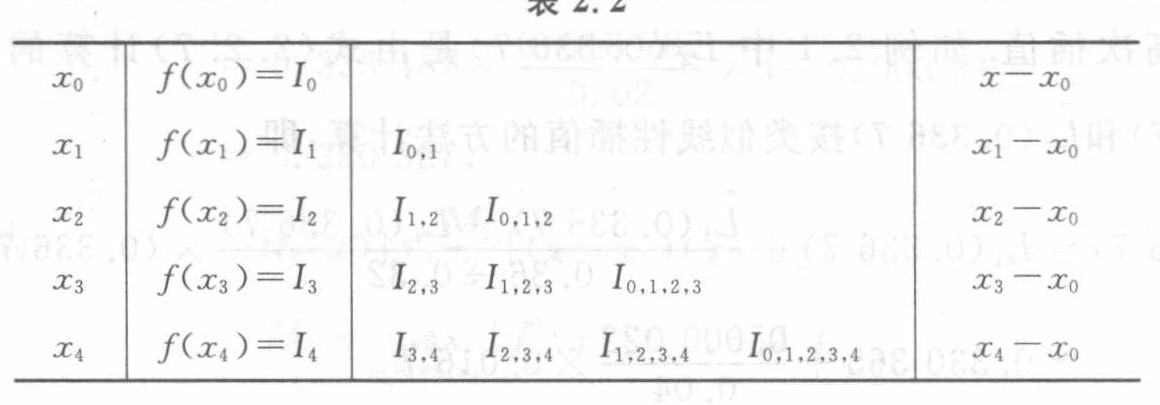
\includegraphics[width=0.85\linewidth,height=\textheight,keepaspectratio,alt={表 2.2 原图核对裁切}]{verified/assets/ch02a/pdf-035-table-2.2-detail.png}

\clearpage

原书 PDF 页 36；印刷页码 23。

\href{source-images/pdf-036.jpeg}{原页：书页 23／PDF 36}

\begin{quote}
页首接 PDF 35 的``插值多项式的''。
\end{quote}

值；如精度不满足要求，再增加一个节点，前面计算完全有效。这个算法适用于在计算机上计算，且具有自动选取节点并逐步比较精度的特点，程序也较简单。

\textbf{例 2.2} 已知 \(f(x)=\operatorname{sh}x\) 的值在表 2.3 左端，用 Aitken 插值求 \(\operatorname{sh}0.23\) 的近似值。

\textbf{解} 表 2.3 右端是各次插值的计算结果，由于 3 次插值的两个结果相同，因而不需再计算 4 次插值，故求得 \(f(0.23)=0.232\,034\)。

\textbf{表 2.3}

\begin{quote}
原表表头为 \(x_i\)、\(f(x_i)\)、插值结果。左右数据在扫描中采用错行排布，以下分开排成可检索表；``1 次、2 次、3 次''为 agent 添加的列名。
\end{quote}

左端节点数据：

{\def\LTcaptype{none} % do not increment counter
\begin{longtable}[]{@{}rr@{}}
\toprule\noalign{}
\(x_i\) & \(f(x_i)\) \\
\midrule\noalign{}
\endhead
\bottomrule\noalign{}
\endlastfoot
\(0.00\) & \(0.000\,0\) \\
\(0.20\) & \(0.201\,34\) \\
\(0.30\) & \(0.304\,52\) \\
\(0.50\) & \(0.521\,10\) \\
\(0.60\) & \(0.636\,65\) \\
\end{longtable}
}

右端插值结果：

{\def\LTcaptype{none} % do not increment counter
\begin{longtable}[]{@{}rrr@{}}
\toprule\noalign{}
1 次 & 2 次 & 3 次 \\
\midrule\noalign{}
\endhead
\bottomrule\noalign{}
\endlastfoot
\(0.231\,54\) & & \\
\(0.233\,465\) & \(0.232\,118\) & \\
\(0.239\,706\) & \(0.232\,358\) & \(\underline{0.232\,034}\) \\
\(0.244\,049\) & \(0.232\,479\) & \(0.232\,034\) \\
\end{longtable}
}

\subsection{2.4 差商与 Newton 插值公式}\label{ch02a-ux5deeux5546ux4e0e-newton-ux63d2ux503cux516cux5f0f}

\subsubsection{2.4.1 差商及其性质}\label{ch02a-ux5deeux5546ux53caux5176ux6027ux8d28}

Lagrange 插值公式可以看作直线方程两点式的推广，如果从点斜式直线方程

\[
P_1(x)=f_0+\frac{f_1-f_0}{x_1-x_0}(x-x_0)
\]

出发，将它推广到具有 \(n+1\) 个插值点 \((x_0,f_0),(x_1,f_1),\cdots,(x_n,f_n)\) 的情况，则可把插值多项式表示为

\[
\begin{aligned}
P_n(x)={}&a_0+a_1(x-x_0)+a_2(x-x_0)(x-x_1)+\cdots\\
&+a_n(x-x_0)\cdots(x-x_{n-1}),
\end{aligned}
\tag{2.4.1}
\]

其中 \(a_0,a_1,\cdots,a_n\) 为待定系数，可由插值条件 \(P_n(x_j)=f_j\;(j=0,1,\cdots,n)\) 确定。

当 \(x=x_0\) 时，\(P_n(x_0)=a_0=f_0\)；当 \(x=x_1\) 时，\(P_n(x_1)=a_0+a_1(x-x_0)=f_1\)，推得

\[
a_1=\frac{f_1-f_0}{x_1-x_0};
\]

当 \(x=x_2\) 时，\(P_n(x_2)=a_0+a_1(x_2-x_0)+a_2(x_2-x_0)(x_2-x_1)=f_2\)，

推得

\[
a_2=\frac{\dfrac{f_2-f_0}{x_2-x_0}-\dfrac{f_1-f_0}{x_1-x_0}}{x_2-x_1}.
\]

依此递推，可得到 \(a_3,a_4,\cdots,a_n\)。为写出系数 \(a_k\) 的一般表达式，先引进如下差商定义。

\textbf{定义 2.3} 称 \(f[x_0,x_k]=\dfrac{f(x_k)-f(x_0)}{x_k-x_0}\) 为函数 \(f(x)\) 关于点 \(x_0,x_k\) 的一阶差商，称

\begin{quote}
定义 2.3 续 PDF 37。
\end{quote}

\subsubsection{校注（agent 补充）：代入行的原书记号}\label{ch02a-ux6821ux6ce8agent-ux8865ux5145ux4ee3ux5165ux884cux7684ux539fux4e66ux8bb0ux53f7}

上面``当 \(x=x_1\) 时''一行，扫描原书实际写成 \(a_0+a_1(x-x_0)\)，其中 \(x\) 没有下标 \(1\)，本转录予以保留。在该行已经限定的 \(x=x_1\) 条件下，求系数时即代入 \(x_1\)；不将这一记号静默改写成原文没有印出的 \(a_1(x_1-x_0)\)。原页的 \(a_2\) 分式有整体分母 \(x_2-x_1\)，OCR 漏掉了这一层分母，本转录已恢复。

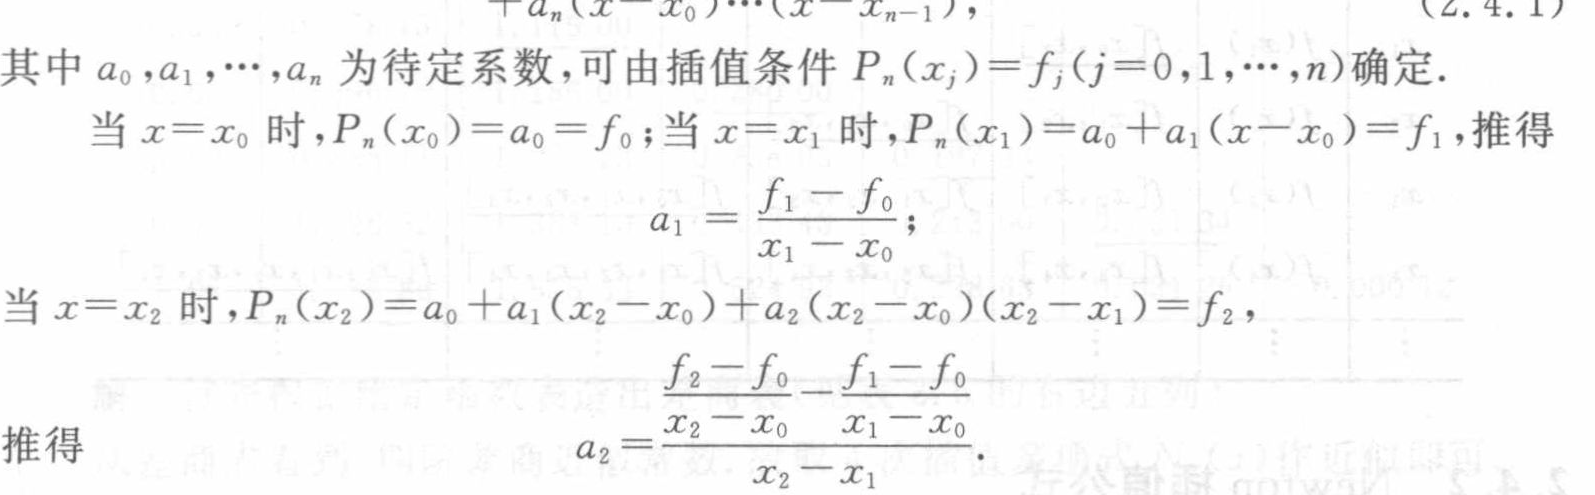
\includegraphics[width=0.85\linewidth,height=\textheight,keepaspectratio,alt={PDF 36 代入与系数原图裁切}]{verified/assets/ch02a/pdf-036-coefficients-detail.png}

\clearpage

原书 PDF 页 37；印刷页码 24。

\href{source-images/pdf-037.jpeg}{原页：书页 24／PDF 37}

\begin{quote}
页首承接 PDF 36 的定义 2.3；页末递推式续 PDF 38。
\end{quote}

\[
f[x_0,x_1,x_k]=\frac{f[x_0,x_k]-f[x_0,x_1]}{x_k-x_1}
\]

为 \(f(x)\) 关于点 \(x_0,x_1,x_k\) 的二阶差商。一般地，称

\[
f[x_0,x_1,\cdots,x_k]=\frac{f[x_0,x_1,\cdots,x_{k-2},x_k]-f[x_0,x_1,\cdots,x_{k-1}]}{x_k-x_{k-1}}
\tag{2.4.2}
\]

为 \(f(x)\) 的 \(k\) 阶差商。

差商有如下的基本性质：

（1）\(k\) 阶差商可表示为函数值 \(f(x_0),f(x_1),\cdots,f(x_k)\) 的线性组合，即

\[
f[x_0,x_1,\cdots,x_k]=\sum_{j=0}^{k}\frac{f(x_j)}{(x_j-x_0)\cdots(x_j-x_{j-1})(x_j-x_{j+1})\cdots(x_j-x_k)}.
\tag{2.4.3}
\]

这个性质可用归纳法证明。这个性质也表明差商与节点的排列次序无关，称为差商的对称性，即

\[
f[x_0,x_1,\cdots,x_k]=f[x_1,x_0,x_2,\cdots,x_k]=\cdots=f[x_1,x_2,\cdots,x_k,x_0].
\]

（2）由性质（1）及式（2.4.2）可得

\[
f[x_0,x_1,\cdots,x_k]=\frac{f[x_1,x_2,\cdots,x_k]-f[x_0,x_1,\cdots,x_{k-1}]}{x_k-x_0}.
\tag{2.4.4}
\]

（3）若 \(f(x)\) 在 \([a,b]\) 上存在 \(n\) 阶导数，且节点 \(x_0,x_1,\cdots,x_n\in[a,b]\)，则 \(n\) 阶差商与导数关系为

\[
f[x_0,x_1,\cdots,x_n]=\frac{f^{(n)}(\xi)}{n!},\qquad\xi\in[a,b].
\tag{2.4.5}
\]

这个公式可直接用 Rolle 定理证明。

差商的其他性质还可见本章习题。差商计算可列差商表如表 2.4 所示。

\textbf{表 2.4}

{\def\LTcaptype{none} % do not increment counter
\begin{longtable}[]{@{}
  >{\raggedright\arraybackslash}p{(\linewidth - 10\tabcolsep) * \real{0.1667}}
  >{\raggedright\arraybackslash}p{(\linewidth - 10\tabcolsep) * \real{0.1667}}
  >{\raggedright\arraybackslash}p{(\linewidth - 10\tabcolsep) * \real{0.1667}}
  >{\raggedright\arraybackslash}p{(\linewidth - 10\tabcolsep) * \real{0.1667}}
  >{\raggedright\arraybackslash}p{(\linewidth - 10\tabcolsep) * \real{0.1667}}
  >{\raggedright\arraybackslash}p{(\linewidth - 10\tabcolsep) * \real{0.1667}}@{}}
\toprule\noalign{}
\begin{minipage}[b]{\linewidth}\raggedright
\(x_k\)
\end{minipage} & \begin{minipage}[b]{\linewidth}\raggedright
\(f(x_k)\)
\end{minipage} & \begin{minipage}[b]{\linewidth}\raggedright
一阶差商
\end{minipage} & \begin{minipage}[b]{\linewidth}\raggedright
二阶差商
\end{minipage} & \begin{minipage}[b]{\linewidth}\raggedright
三阶差商
\end{minipage} & \begin{minipage}[b]{\linewidth}\raggedright
四阶差商
\end{minipage} \\
\midrule\noalign{}
\endhead
\bottomrule\noalign{}
\endlastfoot
\(x_0\) & \(\underline{f(x_0)}\) & & & & \\
\(x_1\) & \(f(x_1)\) & \(\underline{f[x_0,x_1]}\) & & & \\
\(x_2\) & \(f(x_2)\) & \(f[x_1,x_2]\) & \(\underline{f[x_0,x_1,x_2]}\) & & \\
\(x_3\) & \(f(x_3)\) & \(f[x_2,x_3]\) & \(f[x_1,x_2,x_3]\) & \(\underline{f[x_0,x_1,x_2,x_3]}\) & \\
\(x_4\) & \(f(x_4)\) & \(f[x_3,x_4]\) & \(f[x_2,x_3,x_4]\) & \(f[x_1,x_2,x_3,x_4]\) & \(\underline{f[x_0,x_1,x_2,x_3,x_4]}\) \\
\(\vdots\) & \(\vdots\) & \(\vdots\) & \(\vdots\) & \(\vdots\) & \(\vdots\) \\
\end{longtable}
}

\subsubsection{2.4.2 Newton 插值公式}\label{ch02a-newton-ux63d2ux503cux516cux5f0f}

根据差商定义，把 \(x\) 看成 \([a,b]\) 上一点，可得

\[
f(x)=f(x_0)+f[x,x_0](x-x_0),
\]

\clearpage

原书 PDF 页 38；印刷页码 25。

\href{source-images/pdf-038.jpeg}{原页：书页 25／PDF 38}

\begin{quote}
页首承接 PDF 37 的递推式；本页例 2.3 的计算结果续 PDF 39。
\end{quote}

\[
\begin{aligned}
f[x,x_0]&=f[x_0,x_1]+f[x,x_0,x_1](x-x_1),\\
&\vdots\\
f[x,x_0,\cdots,x_{n-1}]&=f[x_0,x_1,\cdots,x_n]+f(x,x_0,\cdots,x_n](x-x_n).
\end{aligned}
\]

只要把后一式代入前一式，就可得到

\[
\begin{aligned}
f(x)={}&f(x_0)+f[x_0,x_1](x-x_0)+f[x_0,x_1,x_2](x-x_0)(x-x_1)+\cdots\\
&+f[x_0,x_1,\cdots,x_n](x-x_0)\cdots(x-x_{n-1})+f[x,x_0,\cdots,x_n]\omega_{n+1}(x)\\
={}&N_n(x)+R_n(x),
\end{aligned}
\]

其中

\[
\begin{aligned}
N_n(x)={}&f(x_0)+f[x_0,x_1](x-x_0)+f[x_0,x_1,x_2](x-x_0)(x-x_1)+\cdots\\
&+f[x_0,x_1,\cdots,x_n](x-x_0)(x-x_1)\cdots(x-x_{n-1}),
\end{aligned}
\tag{2.4.6}
\]

\[
R_n(x)=f(x)-N_n(x)=f[x,x_0,\cdots,x_n]\omega_{n+1}(x).
\tag{2.4.7}
\]

\(\omega_{n+1}(x)\) 是由式（2.2.12）定义的。由式（2.4.6）确定的多项式 \(N_n(x)\) 显然满足插值条件，且次数不超过 \(n\)，它就是形如式（2.4.1）的多项式，其系数为

\[
a_k=f[x_0,x_1,\cdots,x_k]\qquad(k=0,1,\cdots,n).
\]

称 \(N_n(x)\) 为 \textbf{Newton 差商插值多项式}。系数 \(a_k\) 就是差商表 2.4 中加横线的各阶差商，它比 Lagrange 插值节省计算量，且便于程序设计。

式（2.4.7）为插值余项，由插值多项式的唯一性知，它与式（2.2.14）是等价的，事实上，利用差商与导数关系式（2.4.5），可由式（2.4.7）推出式（2.2.14）。但式（2.4.7）更有一般性，它对于 \(f\) 是由离散点给出的情形或 \(f\) 导数不存在时均适用。

\textbf{例 2.3} 给出 \(f(x)\) 的函数表（见表 2.5 左边两列），求 4 次 Newton 插值多项式，并由此计算 \(f(0.596)\) 的近似值。

\textbf{表 2.5}

{\def\LTcaptype{none} % do not increment counter
\begin{longtable}[]{@{}
  >{\raggedright\arraybackslash}p{(\linewidth - 12\tabcolsep) * \real{0.1429}}
  >{\raggedright\arraybackslash}p{(\linewidth - 12\tabcolsep) * \real{0.1429}}
  >{\raggedright\arraybackslash}p{(\linewidth - 12\tabcolsep) * \real{0.1429}}
  >{\raggedright\arraybackslash}p{(\linewidth - 12\tabcolsep) * \real{0.1429}}
  >{\raggedright\arraybackslash}p{(\linewidth - 12\tabcolsep) * \real{0.1429}}
  >{\raggedright\arraybackslash}p{(\linewidth - 12\tabcolsep) * \real{0.1429}}
  >{\raggedright\arraybackslash}p{(\linewidth - 12\tabcolsep) * \real{0.1429}}@{}}
\toprule\noalign{}
\begin{minipage}[b]{\linewidth}\raggedright
\(x_k\)
\end{minipage} & \begin{minipage}[b]{\linewidth}\raggedright
\(f(x_k)\)
\end{minipage} & \begin{minipage}[b]{\linewidth}\raggedright
一阶差商
\end{minipage} & \begin{minipage}[b]{\linewidth}\raggedright
二阶差商
\end{minipage} & \begin{minipage}[b]{\linewidth}\raggedright
三阶差商
\end{minipage} & \begin{minipage}[b]{\linewidth}\raggedright
四阶差商
\end{minipage} & \begin{minipage}[b]{\linewidth}\raggedright
五阶差商
\end{minipage} \\
\midrule\noalign{}
\endhead
\bottomrule\noalign{}
\endlastfoot
\(0.40\) & \(\underline{0.410\,75}\) & & & & & \\
\(0.55\) & \(0.578\,15\) & \(\underline{1.116\,00}\) & & & & \\
\(0.65\) & \(0.696\,75\) & \(1.186\,00\) & \(\underline{0.280\,00}\) & & & \\
\(0.80\) & \(0.888\,11\) & \(1.275\,73\) & \(0.358\,93\) & \(\underline{0.197\,33}\) & & \\
\(0.90\) & \(1.026\,52\) & \(1.384\,10\) & \(0.433\,48\) & \(0.213\,00\) & \(\underline{0.031\,34}\) & \\
\(1.05\) & \(1.253\,82\) & \(1.515\,33\) & \(0.524\,93\) & \(0.228\,63\) & \(0.031\,26\) & \(-0.000\,12\) \\
\end{longtable}
}

\textbf{解} 首先根据给定函数表造出差商表（见表 2.5 的右边五列）。

从差商表看到，四阶差商近似常数。故取 4 次插值多项式 \(N_4(x)\) 作近似即可。

\[
\begin{aligned}
N_4(x)={}&0.410\,75+1.116(x-0.4)+0.28(x-0.4)(x-0.55)\\
&+0.197\,33(x-0.4)(x-0.55)(x-0.65)\\
&+0.031\,34(x-0.4)(x-0.55)(x-0.65)(x-0.8),
\end{aligned}
\]

\subsubsection{校注（agent 补充）：CH02A-S01，差商的左括号}\label{ch02a-ux6821ux6ce8agent-ux8865ux5145ch02a-s01ux5deeux5546ux7684ux5de6ux62ecux53f7}

本页页首递推式的最后一项，原书印为 \(f(x,x_0,\cdots,x_n]\)，左右括号不配。本转录保留这一印字。根据定义 2.3、同页后续两式及差商记号，此处应理解为 \(f[x,x_0,\cdots,x_n]\)；这是原书排印问题，不是 OCR 错误。CH02A-S01 是本 lane 的临时校注编号。

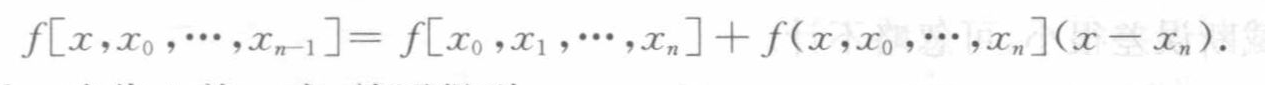
\includegraphics[width=0.85\linewidth,height=\textheight,keepaspectratio,alt={差商括号原图裁切}]{verified/assets/ch02a/pdf-038-recurrence-detail.png}

\subsubsection{校注（agent 补充）：CH02A-S03，表 2.5 的中间舍入}\label{ch02a-ux6821ux6ce8agent-ux8865ux5145ch02a-s03ux8868-2.5-ux7684ux4e2dux95f4ux820dux5165}

上表按原书印字转录。若把左端两列所给小数作为精确输入，使用差商递推且保留精确分数，则第三个二阶差商为 \(0.433466666\cdots\)，四阶差商分别为 \(0.031238095\cdots\)、\(0.031428571\cdots\)，五阶差商为 \(2/6825=0.000293040293\cdots\)；它们与表中 \(0.43348\)、\(0.03134\)、\(0.03126\)、\(-0.00012\) 不同。

逐列检查表明：表中 \(0.43348\) 可以由已舍入的一阶差商重算得到，而 \(0.35893\)、\(0.52493\) 更接近保留未舍入一阶差商的计算；原表的三至五阶差商则能从其已印出的前一列经舍入重算得到。因此，本例高阶差商对中间舍入敏感，不能把这张有限精度表当作精确差商表。此处记录的是原书数值计算的舍入一致性问题，不修改原表。

\clearpage

原书 PDF 页 39；印刷页码 26。

\href{source-images/pdf-039.jpeg}{原页：书页 26／PDF 39}

\begin{quote}
页首为 PDF 38 例 2.3 的续算；页末性质 1 的公式续 PDF 40。
\end{quote}

于是

\[
f(0.596)\approx N_4(0.596)=0.631\,95.
\]

截断误差

\[
|R_4(x)|\approx|f[x_0,x_1,\cdots,x_5]\omega_5(0.596)|\le3.63\times10^{-9}.
\]

这说明截断误差很小，可忽略不计。

\subsection{2.5 差分与等距节点插值公式}\label{ch02a-ux5deeux5206ux4e0eux7b49ux8dddux8282ux70b9ux63d2ux503cux516cux5f0f}

上面讨论了节点任意分布的插值公式，但实际应用时经常遇到等距节点的情形，这时插值公式可以进一步简化，计算也简单得多。为了得到等距节点的插值公式，下面先介绍差分的概念。

\subsubsection{2.5.1 差分及其性质}\label{ch02a-ux5deeux5206ux53caux5176ux6027ux8d28}

设函数 \(y=f(x)\) 在等距节点 \(x_k=x_0+kh\;(k=0,1,\cdots,n)\) 上的值 \(f_k=f(x_k)\) 为已知，这里 \(h\) 为常数，称为\textbf{步长}。

\textbf{定义 2.4} 偏差

\[
\Delta f_k=f_{k+1}-f_k,
\tag{2.5.1}
\]

\[
\nabla f_k=f_k-f_{k-1},
\tag{2.5.2}
\]

\[
\delta f_k=f(x_k+h/2)-f(x_k-h/2)=f_{k+\frac12}-f_{k-\frac12}
\tag{2.5.3}
\]

分别称为 \(f(x)\) 在 \(x_k\) 处以 \(h\) 为步长的\textbf{向前差分}、\textbf{向后差分}及\textbf{中心差分}。符号 \(\Delta,\nabla,\delta\) 分别称为\textbf{向前差分算子}、\textbf{向后差分算子}及\textbf{中心差分算子}。

利用一阶差分可定义二阶差分为

\[
\Delta^2 f_k=\Delta f_{k+1}-\Delta f_k=f_{k+2}-2f_{k+1}+f_k.
\]

一般地，可定义 \(m\) 阶差分为

\[
\Delta^m f_k=\Delta^{m-1}f_{k+1}-\Delta^{m-1}f_k,\qquad
\nabla^m f_k=\nabla^{m-1}f_k-\nabla^{m-1}f_{k-1}.
\]

因中心差分 \(\delta f_k\) 用到 \(f_{k+\frac12}\) 及 \(f_{k-\frac12}\) 这两个值，实际上不是函数表上的值。如果用函数表上的值，一阶中心差分应写成

\[
\delta f_{k+\frac12}=f_{k+1}-f_k,\qquad
\delta f_{k-\frac12}=f_k-f_{k-1};
\]

二阶中心差分为 \(\delta^2 f_k=\delta f_{k+\frac12}-\delta f_{k-\frac12}\)；等等。

除了已引入的差分算子外，常用算子符号还有\textbf{不变算子 \(\mathrm{I}\)} 及\textbf{移位算子 \(\mathrm{E}\)}，定义如下：

\[
\mathrm{I}f_k=f_k,\qquad\mathrm{E}f_k=f_{k+1},
\]

于是，由 \(\Delta f_k=f_{k+1}-f_k=\mathrm{E}f_k-\mathrm{I}f_k=(\mathrm{E}-\mathrm{I})f_k\)，可得 \(\Delta=\mathrm{E}-\mathrm{I}\)。

同理，可得

\[
\nabla=\mathrm{I}-\mathrm{E}^{-1},\qquad
\delta=\mathrm{E}^{\frac12}-\mathrm{E}^{-\frac12}.
\]

由差分定义并应用算子符号运算可得下列基本性质。

\textbf{性质 1} 各阶差分均可用函数值表示。例如

\subsubsection{校注（agent 补充）：例 2.3 的误差估计范围}\label{ch02a-ux6821ux6ce8agent-ux8865ux5145ux4f8b-2.3-ux7684ux8befux5deeux4f30ux8ba1ux8303ux56f4}

页首 \(3.63\times10^{-9}\) 使用原表 2.5 的五阶差商 \(-0.00012\) 及乘积 \(\omega_5(0.596)\) 得到，原文已使用近似号。原表高阶差商的舍入敏感性见 PDF 38 校注 CH02A-S03；仅凭给定的有限节点表值，不能对任意与这些节点相符的函数证明这一截断误差上界，节点数据的舍入误差也未计入。以上是 agent 的适用范围说明，原书结论仍在正文保留。

\subsubsection{校注（agent 补充）：CH02A-S04，例 2.3 的函数值结果}\label{ch02a-ux6821ux6ce8agent-ux8865ux5145ch02a-s04ux4f8b-2.3-ux7684ux51fdux6570ux503cux7ed3ux679c}

原书本页实际印为 \(N_4(0.596)=0.63195\)，本转录保留该数。按 PDF 38 原印的四次多项式逐项代入 \(x=0.596\)，得到

\[
N_4(0.596)=0.63191751982370304,
\]

保留五位小数为 \(0.63192\)，与原书的 \(0.63195\) 不符。这一差异并非末位舍入造成，属于原书该计算结果的数值错误。

\clearpage

原书 PDF 页 40；印刷页码 27。

\href{source-images/pdf-040.jpeg}{原页：书页 27／PDF 40}

\begin{quote}
页首承接 PDF 39 的性质 1。
\end{quote}

\[
\Delta^n f_k=(\mathrm{E}-\mathrm{I})^n f_k
=\sum_{j=0}^{n}(-1)^j\binom{n}{j}\mathrm{E}^{n-j}f_k
=\sum_{j=0}^{n}(-1)^j\binom{n}{j}f_{n+k-j},
\tag{2.5.4}
\]

\[
\nabla^n f_k=(\mathrm{I}-\mathrm{E}^{-1})^n f_k
=\sum_{j=0}^{n}(-1)^{n-j}\binom{n}{j}\mathrm{E}^{j-n}f_k
=\sum_{j=0}^{n}(-1)^{n-j}\binom{n}{j}f_{k+j-n},
\tag{2.5.5}
\]

其中 \(\displaystyle\binom{n}{j}=\frac{n(n-1)\cdots(n-j+1)}{j!}\) 为二项式展开系数。

\textbf{性质 2} 可用各阶差分表示函数值，例如，可用向前差分表示 \(f_{n+k}\)，即

\[
f_{n+k}=\mathrm{E}^n f_k=(\mathrm{I}+\Delta)^n f_k=\sum_{j=0}^{n}\binom{n}{j}\Delta^j f_k.
\tag{2.5.6}
\]

\textbf{性质 3} 差商与差分有以下关系，例如，对于向前差分，由定义

\[
f[x_k,x_{k+1}]=\frac{f_{k+1}-f_k}{x_{k+1}-x_k}=\frac{\Delta f_k}{h},
\]

\[
f[x_k,x_{k+1},x_{k+2}]=\frac{f[x_{k+1},x_{k+2}]-f[x_k,x_{k+1}]}{x_{k+2}-x_k}=\frac{1}{2h^2}\Delta^2 f_k,
\]

一般地有

\[
f[x_k,x_{k+1},\cdots,x_{k+m}]=\frac{1}{m!}\frac{1}{h^m}\Delta^m f_k\qquad(m=1,2,\cdots,n).
\tag{2.5.7}
\]

同理，对于向后差分，有

\[
f[x_k,x_{k-1},\cdots,x_{k-m}]=\frac{1}{m!}\frac{1}{h^m}\nabla^m f_k.
\tag{2.5.8}
\]

利用式（2.5.7）及式（2.4.5）又可得到

\[
\Delta^n f_k=h^n f^{(n)}(\xi),
\tag{2.5.9}
\]

其中 \(\xi\in(x_k,x_{k+n})\)，这是差分与导数的关系。差分的其他性质可参看习题 10～12。

计算差分可列差分表，表 2.6 是向前差分表。

\textbf{表 2.6}

{\def\LTcaptype{none} % do not increment counter
\begin{longtable}[]{@{}
  >{\raggedright\arraybackslash}p{(\linewidth - 8\tabcolsep) * \real{0.2000}}
  >{\raggedright\arraybackslash}p{(\linewidth - 8\tabcolsep) * \real{0.2000}}
  >{\raggedright\arraybackslash}p{(\linewidth - 8\tabcolsep) * \real{0.2000}}
  >{\raggedright\arraybackslash}p{(\linewidth - 8\tabcolsep) * \real{0.2000}}
  >{\raggedright\arraybackslash}p{(\linewidth - 8\tabcolsep) * \real{0.2000}}@{}}
\toprule\noalign{}
\begin{minipage}[b]{\linewidth}\raggedright
\(x_k\)
\end{minipage} & \begin{minipage}[b]{\linewidth}\raggedright
\(\Delta\)
\end{minipage} & \begin{minipage}[b]{\linewidth}\raggedright
\(\Delta^2\)
\end{minipage} & \begin{minipage}[b]{\linewidth}\raggedright
\(\Delta^3\)
\end{minipage} & \begin{minipage}[b]{\linewidth}\raggedright
\(\Delta^4\)
\end{minipage} \\
\midrule\noalign{}
\endhead
\bottomrule\noalign{}
\endlastfoot
\(f_0\) & \(\Delta f_0\) & \(\Delta^2 f_0\) & \(\Delta^3 f_0\) & \(\Delta^4 f_0\) \\
\(f_1\) & \(\Delta f_1\) & \(\Delta^2 f_1\) & \(\Delta^3 f_1\) & \(\vdots\) \\
\(f_2\) & \(\Delta f_2\) & \(\Delta^2 f_2\) & \(\vdots\) & \\
\(f_3\) & \(\Delta f_3\) & \(\vdots\) & & \\
\(f_4\) & \(\vdots\) & & & \\
\(\vdots\) & & & & \\
\end{longtable}
}

\subsubsection{校注（agent 补充）：CH02A-S02，表 2.6 的首列表头}\label{ch02a-ux6821ux6ce8agent-ux8865ux5145ch02a-s02ux8868-2.6-ux7684ux9996ux5217ux8868ux5934}

原书表 2.6 首列表头实际印为 \(x_k\)，而其内容为 \(f_0,f_1,\cdots\)，本转录均按原图保留。依各阶向前差分的意义，该列存放函数值，表头应理解为 \(f_k\)；这是原书表头与内容不一致的问题。CH02A-S02 是本 lane 的临时校注编号。

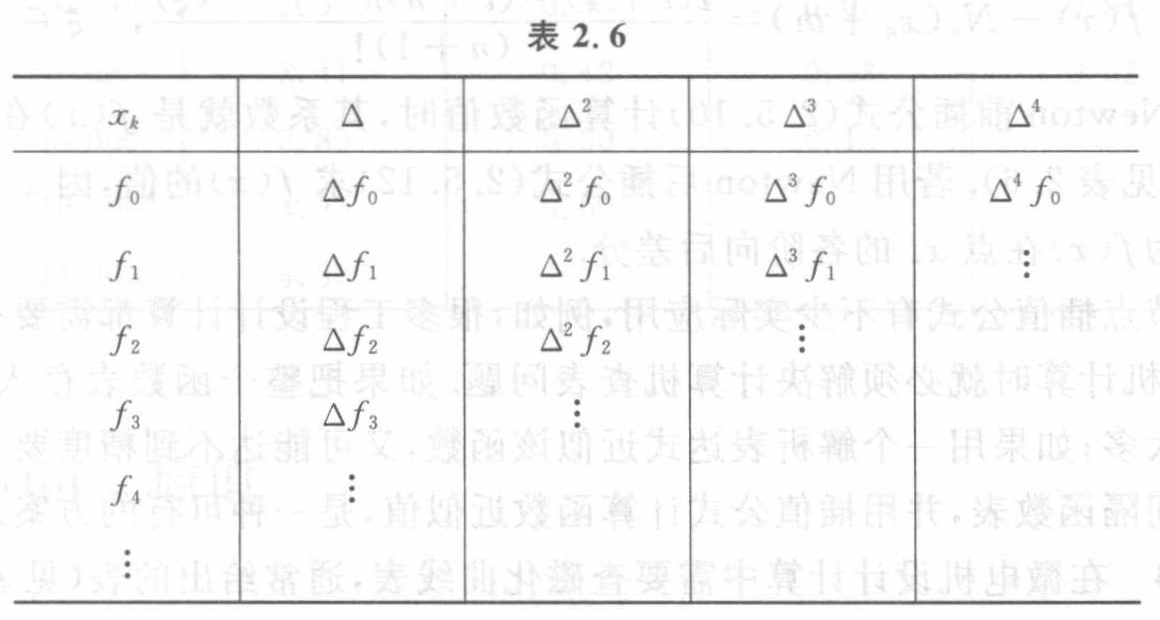
\includegraphics[width=0.85\linewidth,height=\textheight,keepaspectratio,alt={表 2.6 原图裁切}]{verified/assets/ch02a/pdf-040-table-2.6.png}

\clearpage

原书 PDF 页 41；印刷页码 28。

\href{source-images/pdf-041.jpeg}{原页：书页 28／PDF 41}

\subsubsection{2.5.2 等距节点插值公式}\label{ch02a-ux7b49ux8dddux8282ux70b9ux63d2ux503cux516cux5f0f}

将 Newton 差商插值多项式（2.4.6）中各阶差商用相应差分代替，就可得到各种形式的等距节点插值公式。这里只推导常用的前插公式与后插公式。

如果节点 \(x_k=x_0+kh\;(k=0,1,\cdots,n)\)，要计算 \(x_0\) 附近点 \(x\) 的函数 \(f(x)\) 的值，可令 \(x=x_0+th\)，\(0\le t\le1\)，于是

\[
\omega_{k+1}(x)=\prod_{j=0}^{k}(x-x_j)=t(t-1)\cdots(t-k)h^{k+1}.
\]

将此式及式（2.5.7）代入式（2.4.6），得

\[
N_n(x_0+th)=f_0+t\Delta f_0+\frac{t(t-1)}{2!}\Delta^2 f_0+\cdots+\frac{t(t-1)\cdots(t-n+1)}{n!}\Delta^n f_0.
\tag{2.5.10}
\]

式（2.5.10）称为 \textbf{Newton 前插公式}，其余项由式（2.2.14）得

\[
R_n(x)=\frac{t(t-1)\cdots(t-n)}{(n+1)!}h^{n+1}f^{(n+1)}(\xi),\qquad\xi\in(x_0,x_n).
\tag{2.5.11}
\]

如果要求表示函数在 \(x_n\) 附近的值 \(f(x)\)，此时应用 Newton 插值公式（2.4.6），插值点应按 \(x_n,x_{n-1},\cdots,x_0\) 的次序排列，有

\[
\begin{aligned}
N_n(x)={}&f(x_n)+f[x_n,x_{n-1}](x-x_n)+f[x_n,x_{n-1},x_{n-2}](x-x_n)(x-x_{n-1})\\
&+\cdots+f[x_n,x_{n-1},\cdots,x_0](x-x_n)\cdots(x-x_1).
\end{aligned}
\]

作变换 \(x=x_n+th\;(-1\le t\le0)\)，并利用式（2.5.8），代入上式得

\[
\begin{aligned}
N_n(x_n+th)={}&f_n+t\nabla f_n+\frac{t(t+1)}{2!}\nabla^2 f_n+\cdots\\
&+\frac{t(t+1)\cdots(t+n-1)}{n!}\nabla^n f_n.
\end{aligned}
\tag{2.5.12}
\]

式（2.5.12）称为 \textbf{Newton 后插公式}，其余项

\[
R_n(x)=f(x)-N_n(x_n+th)=\frac{t(t+1)\cdots(t+n)h^{n+1}f^{(n+1)}(\xi)}{(n+1)!},\qquad\xi\in(x_0,x_n).
\]

利用 Newton 前插公式（2.5.10）计算函数值时，其系数就是 \(f(x)\) 在 \(x_0\) 的各阶向前差分（见表 2.6）。若用 Newton 后插公式（2.5.12）求 \(f(x)\) 的值，因 \(x\) 在 \(x_n\) 附近，则其系数为 \(f(x)\) 在点 \(x_n\) 的各阶向后差分。

等距节点插值公式有不少实际应用，例如，很多工程设计计算都需要查各种函数表，用计算机计算时就必须解决计算机查表问题。如果把整个函数表存入内存，往往占用单元太多；如果用一个解析表达式近似该函数，又可能达不到精度要求。因此，采用存放大间隔函数表，并用插值公式计算函数近似值，是一种可行的方案。

\textbf{例 2.4} 在微电机设计计算中需要查磁化曲线表，通常给出的表（见表 2.7）是磁密 \(B\) 每间隔 100 高斯磁路每厘米长所需安匝数 \(at\) 的值，下面要解决 \(B\) 从 \(4\,000\) 至

\begin{quote}
例 2.4 的区间上限及解答续 PDF 42。
\end{quote}

\clearpage

原书 PDF 页 42；印刷页码 29。

\href{source-images/pdf-042.jpeg}{原页：书页 29／PDF 42}

\begin{quote}
页首接 PDF 41 例 2.4 的区间；页末 2.6 首句续 PDF 43。
\end{quote}

\(11\,000\) 区间的查表问题。

\textbf{解} 为节省计算机存储单元，采用每 500 高斯存入一个 \(at\) 值。为了分析使用几阶插值公式合适，应先列出差分表。表 2.7 是以硅钢片的磁化曲线为例所造的差分表。

从差分表中看到三阶差分近似于 0，因此计算时只需用二阶差分，当 \(4\,000\le B\le10\,500\) 时用 Newton 前插公式，当 \(10\,500<B\le11\,000\) 时用 Newton 后插公式。例如，求 \(f(5\,200)\) 时取 \(B_0=5\,000\)，\(f_0=1.58\)，\(\Delta f_0=0.11\)，\(\Delta^2 f_0=0.01\)，\(h=500\)，\(B=5\,200\)，\(t=0.4\)，于是由式（2.5.10），取 \(n=2\)，得

\[
f(5\,200)\approx1.58+0.4\times0.11+\frac{0.4\times(-0.6)}{2}\times0.01\approx1.62.
\]

这个结果与直接查表得到的值相同，说明用此法在计算机上求 \(at\) 值是可行的。具体的查表程序作为练习由读者完成。

\textbf{表 2.7}

{\def\LTcaptype{none} % do not increment counter
\begin{longtable}[]{@{}
  >{\raggedleft\arraybackslash}p{(\linewidth - 10\tabcolsep) * \real{0.1667}}
  >{\raggedleft\arraybackslash}p{(\linewidth - 10\tabcolsep) * \real{0.1667}}
  >{\raggedleft\arraybackslash}p{(\linewidth - 10\tabcolsep) * \real{0.1667}}
  >{\raggedleft\arraybackslash}p{(\linewidth - 10\tabcolsep) * \real{0.1667}}
  >{\raggedleft\arraybackslash}p{(\linewidth - 10\tabcolsep) * \real{0.1667}}
  >{\raggedleft\arraybackslash}p{(\linewidth - 10\tabcolsep) * \real{0.1667}}@{}}
\toprule\noalign{}
\begin{minipage}[b]{\linewidth}\raggedleft
\(k\)
\end{minipage} & \begin{minipage}[b]{\linewidth}\raggedleft
\(B_k\)
\end{minipage} & \begin{minipage}[b]{\linewidth}\raggedleft
\(at_k=f(B_k)\)
\end{minipage} & \begin{minipage}[b]{\linewidth}\raggedleft
\(\Delta f_k\)
\end{minipage} & \begin{minipage}[b]{\linewidth}\raggedleft
\(\Delta^2 f_k\)
\end{minipage} & \begin{minipage}[b]{\linewidth}\raggedleft
\(\Delta^3 f_k\)
\end{minipage} \\
\midrule\noalign{}
\endhead
\bottomrule\noalign{}
\endlastfoot
\(0\) & \(4\,000\) & \(1.38\) & \(0.10\) & \(0\) & \(0.01\) \\
\(1\) & \(4\,500\) & \(1.48\) & \(0.10\) & \(0.01\) & \(0\) \\
\(2\) & \(5\,000\) & \(1.58\) & \(0.11\) & \(0.01\) & \(0\) \\
\(3\) & \(5\,500\) & \(1.69\) & \(0.12\) & \(0.01\) & \(0.02\) \\
\(4\) & \(6\,000\) & \(1.81\) & \(0.13\) & \(0.03\) & \(-0.01\) \\
\(5\) & \(6\,500\) & \(1.94\) & \(0.16\) & \(0.02\) & \(0.02\) \\
\(6\) & \(7\,000\) & \(2.10\) & \(0.18\) & \(0.04\) & \(0\) \\
\(7\) & \(7\,500\) & \(2.28\) & \(0.22\) & \(0.04\) & \(0\) \\
\(8\) & \(8\,000\) & \(2.50\) & \(0.26\) & \(0.04\) & \(0.01\) \\
\(9\) & \(8\,500\) & \(2.76\) & \(0.30\) & \(0.05\) & \(0.02\) \\
\(10\) & \(9\,000\) & \(3.06\) & \(0.35\) & \(0.07\) & \(0.01\) \\
\(11\) & \(9\,500\) & \(3.41\) & \(0.42\) & \(0.08\) & \(0.02\) \\
\(12\) & \(10\,000\) & \(3.83\) & \(0.50\) & \(0.10\) & \\
\(13\) & \(10\,500\) & \(4.33\) & \(0.60\) & & \\
\(14\) & \(11\,000\) & \(4.93\) & & & \\
\end{longtable}
}

\subsection{2.6 Hermite 插值}\label{ch02a-hermite-ux63d2ux503c}

不少实际问题不但要求在节点上函数值相等，而且还要求它的导数值相等，甚至

